\subsection{Modelo Conceptual}

\begin{figure}
  \begin{center}
	%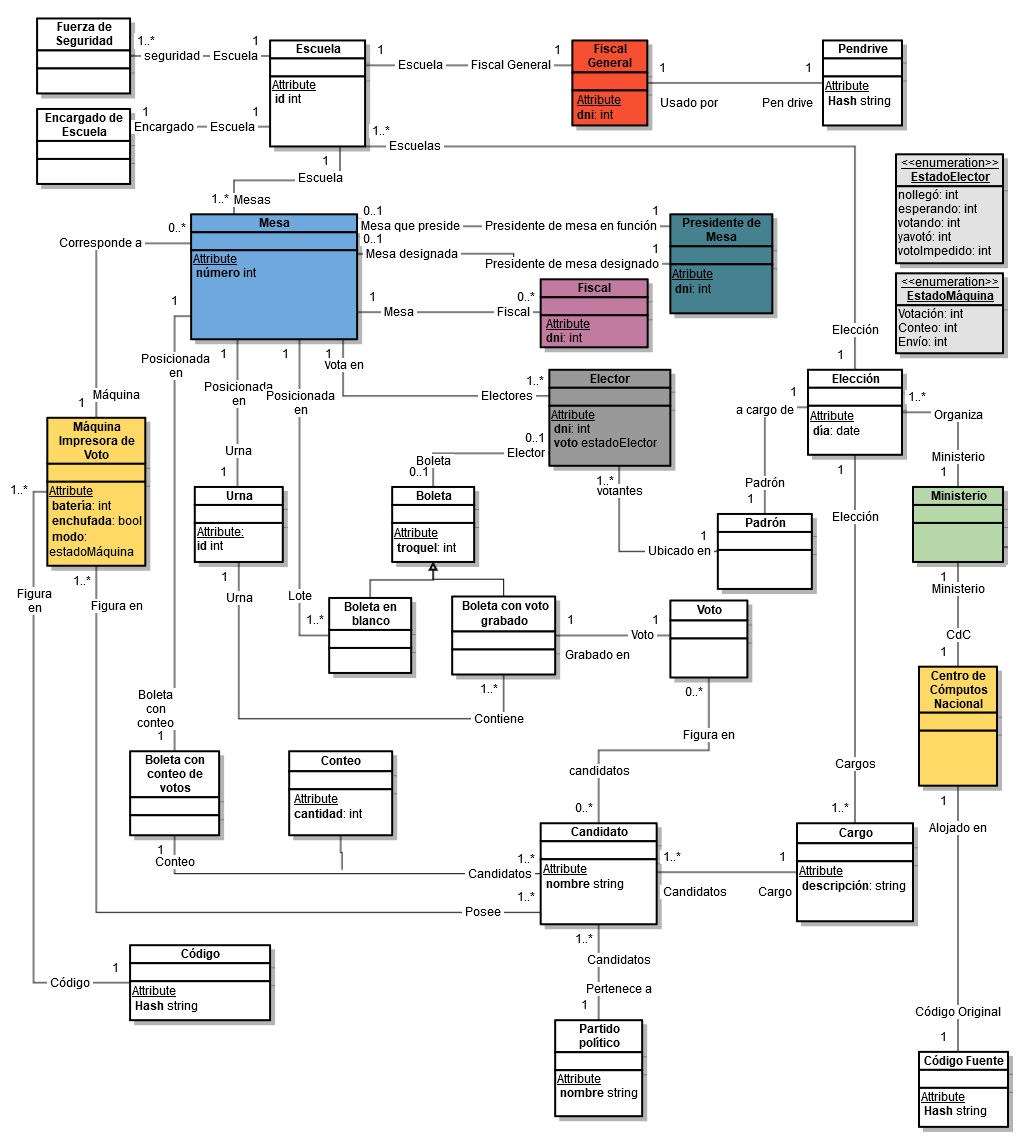
\includegraphics[scale=0.64]{imagenes/clases.png}
  \end{center}
\end{figure}

\newpage
\subsubsection{OCL}


\subsubsection*{Mesa}

\textit{context Mesa
inv}
\begin{enumerate}

\item \textbf{Los n\'umeros de las mesas son únicos.}

$Mesa.AllInstances \rightarrow forAll(m_1, m_2 | m_1.numero <> m_2.numero))$

\item  \textbf{No hay dos mesas con el mismo fiscal.}

$Mesa.AllInstances \rightarrow forAll(m_1, m_2 | m_1.Fiscal.dni <> m_2.Fiscal.dni))$

\item \textbf{No hay dos mesas con electores en común.}

$Mesa.AllInstances \rightarrow \\
 forAll(m_1, m_2 | m_1.Electores \rightarrow \\
 forAll(e_1 | m_2.Electores \rightarrow Select(e_2 | e_1.dni==e_2.dni) \rightarrow Size() == 0))$

\item \textbf{No hay dos mesas con el mismo presidente de mesa.}

$Mesa.AllInstances \rightarrow \\
forAll(m_1, m_2 | m_1.PresidenteDeMesaDesignado.dni <> m_2.PresidenteDeMesaDesignado.dni))$

\item \textbf{Los presidentes de mesa votan en la misma mesa que son presidentes.}

$self.Electores \rightarrow Exists(e | self.PresidenteDeMesaDesignado.dni == e.dni)$

\item \textbf{La cantidad de Boletas Sin voto grabado y con voto grabado de la mesa debe ser mayor o igual a la cantidad de electores de dicha mesa.}

$self.Lote \rightarrow Size() + self.Urna.Contiene \rightarrow Size () \geq self.Electores \rightarrow Size()$

\item \textbf{La cantidad de Boletas Con voto grabado de la mesa debe ser menor o igual a la cantidad de electores de dicha mesa.}

$self.Urna.Contiene  \rightarrow  Size() \leq self.Electores \rightarrow Size()$

\item \textbf{Si la máquina está en modo votación es porque s\'olo un elector, o ninguno, está votando (No puede haber dos electores por mesa votando a la vez).}

$self.Maquina.modo == votacion$  IMPLIES  $ \\
self.Electores \rightarrow select(e | e.voto == votando) \rightarrow Size() \leq 1$

\item \textbf{Si la máquina está en modo conteo es porque no hay ningún elector de la mesa votando o esperando para votar.}

$self.Maquina.modo == votacion$  IMPLIES  $ \\
self.Electores \rightarrow \\
select(e | e.voto == votando$ OR $e.voto == esperando) \rightarrow Size() = 0$

\item \textbf{La máquina de la mesa puede estar en modo votación o conteo pero no en envio.}

$self.Maquina.modo <> envio$

\item \textbf{No puede haber un fiscal y un presidente de mesa con el mismo dni.}

$self.Fiscales \rightarrow \\
select(f | f.dni == self.PresidenteDeMesaEnFuncion.dni OR \\
f.dni == self.PresidenteDeMesaDesignado.dni) \rightarrow \\
Size() == 0 $

\item \textbf{Todos los candidatos de la elecci\'on est\'an en la boleta de conteo de votos (incluyendo cuando la cantidad de votos recibida por el candidato en esa mesa fuese 0).}

$self.Escuela.Eleccion.Cargos \rightarrow \\
forAll(car | car.Candidatos \rightarrow \\
forAll(can_1 | self.BoletaConConteo.Candidatos \rightarrow \\
Exists(can_2| can_1.nombre == can_2.nombre $ AND $car.descripcion==can_2.cargo.descripcion)))$

\item \textbf{\textcolor{red}{El hash del código es el mismo del hash del código fuente. }  }
\item \textbf{\textcolor{red}{El hash del código es el mismo del hash de todos los pendrives de los fiscales.}}


\item \textbf{Si alg\'un elector vot\'o, debe haber votado el presidente mesa antes.}

$self.Electores \rightarrow \\
Exists (e | e.dni <> self.PresidenteDeMesaEnFuncion.dni $ AND $e.voto==yavoto)$ IMPLIES $\\
self.Electores \rightarrow select(v | v.dni==self.PresidenteDeMesaEnFuncion.dni) \rightarrow \\
forAll(p | p.voto==yavoto)$

\end{enumerate}

\subsubsection*{Boleta}

\textit{context Boleta
inv}

\begin{enumerate}

\item \textbf{Los id de las boletas son únicos.}

$Boleta.AllInstances() \rightarrow forAll(b_1, b_2 | b_1.troquel <> b_2.troquel)$

\item \textbf{La boleta con voto grabado tiene elector.}

$self.IsKindOf?(BoletaConVotoGrabado)$  IMPLIES  $self.Elector \rightarrow Size() == 1 $

\item \textbf{Si un elector tiene una boleta en blanco, entonces esta boleta está en la mesa que el elector vota.}

$self.IsKindOf(BoletaEnBlanco)?$ AND $self.Elector \rightarrow Size() == 1 $ IMPLIES $\\
self.PosicionadaEn.numero == self.Elector.VotaEn.numero$

\item \textbf{Si un elector tiene una boleta con voto grabado, entonces esta boleta está en la urna que el elector vot\'o.}

$self.IsKindOf(BoletaConVotoGrabado)? $  IMPLIES  $\\
self.Urna.PosicionadaEn.numero == self.Elector.VotaEn.numero$

\item \textcolor{red}{Los votos de las boletas son de candidatos de la eleccion q vota el elector. PONERLE A LA CLASE ELECCION UNA FECHA. Aclarar en el informe que esto hace q los votos contabilizados en la boleta de conteo tambien son de la misma eleccion ya q las boletas entre si son consistentes y no hace falta aclararlo extra por ocl}

\end{enumerate}

\subsubsection*{Boleta con Conteo de Votos}

\textit{context Boleta con Conteo de Votos
inv}

\begin{enumerate}
\item \textbf{La boleta con Conteo de votos no tiene candidatos repetidos.}

$self.Candidatos \rightarrow forAll(c_1, c_2| c_1.nombre <> c_2.nombre)$

\end{enumerate}
\subsubsection*{Conteo}

\textit{context Conteo
inv}

\begin{enumerate}

\item \textbf{La boleta con conteo tiene la cantidad de votos que recibi\'o cada candidato en esa mesa.}

$self.Cantidad == \\
self.BoletaConConteodeVotos.mesa.boletaConVotoGrabado \rightarrow \\
select(b | b.voto.candidato  \rightarrow exist(c | c==self.candidato)) \rightarrow size() $

\end{enumerate}

\subsubsection*{Voto}

\textit{context Voto
inv}

\begin{enumerate}
\item \textbf{No tiene dos candidatos con el mismo cargo.}

$self.Candidatos  \rightarrow forAll(c_1, c_2 | c_1.cargo.descripcion <> c_2.cargo.descripcion)$

\item \textbf{No tiene dos candidatos con el mismo nombre.}

$self.Candidatos  \rightarrow forAll(c_1, c_2 | c_1.nombre <> c_2.nombre)$

\end{enumerate}

\subsubsection*{Urna}

\textit{context Urna
inv}

\begin{enumerate}

\item \textbf{En una misma urna no hay dos boletas con el mismo elector.}    

$self.Contiene \rightarrow forAll(b_1, b_2 | b_1.Elector.dni<>b_2.Elector.dni)$

\item \textbf{Los id de las urnas son únicos.}

$Urna.AllInstances() \rightarrow forAll(u_1, u_2|u_1.id<>u_2.id)$
\end{enumerate}

\subsubsection*{Escuela}

\textit{context Escuela
inv}

\begin{enumerate}
\item \textbf{Los n\'umeros de las mesas son únicos.}

$Mesa.AllInstances() \rightarrow forAll(m_1, m_2|m_1.numero<>m_2.numero)$

\end{enumerate}

\subsubsection*{M\'aquina Impresora de Voto}

\textit{context M\'aquina Impresora de Voto
inv}

\begin{enumerate}
\item \textbf{\textcolor{red}{Los candidatos de las m\'aquinas corresponden a los candidatos de la elecci\'on de la mesa en que est\'an posicionadas.}}

\end{enumerate}

\subsubsection*{Elector}

\textit{context Elector
inv}

\begin{enumerate}
\item \textbf{Los dni de los electores son únicos.}

$Elector.AllInstances() \rightarrow forAll(e_1, e_2 | e_1.dni <> e_2.dni)$

\item \textbf{Si el elector no llegó, está esperando o no lo dejaron votar no tiene boleta.}

$self.voto==nollego $ OR $self.voto==yavoto$ OR $self.voto==votoImpedido$ IMPLIES $\\
self.Boleta \rightarrow Size() ==0$

 AND 
 
$self.Boleta \rightarrow Size() ==0$ IMPLIES $\\
self.voto==nollego $ OR $self.voto==yavoto$ OR $self.voto==votoImpedido$

\item \textbf{Si el elector está votando, tiene una boleta en blanco.}

$self.Boleta \rightarrow Size() ==1$ IMPLIES $\\
(self.Boleta.IsKindOf?(BoletaEnBlanco)$ IMPLIES $self.voto==votando$ AND

$self.voto==votando$ IMPLIES $self.Boleta.IsKindOf?(BoletaEnBlanco))$

\item \textbf{Si el elector ya votó, tiene una boleta con voto grabado.}

$self.Boleta \rightarrow Size() ==1$ IMPLIES $\\
(self.Boleta.IsKindOf?(BoletaConVotoGrabado)$ IMPLIES $self.voto==yavoto$ AND

$self.voto==yavoto$ IMPLIES $self.Boleta.IsKindOf?(BoletaConVotoGrabado))$

\end{enumerate}

\subsubsection*{Partido Pol\'itico}

\textit{context Partido Pol\'itico
inv}

\begin{enumerate}
\item \textbf{No hay dos partidos políticos con algún candidato en común.}

$PartidoPolitico.AllInstances() \rightarrow \\
forAll(p_1, p_2 | p_1.candidatos \rightarrow \\
forAll(c_1 | p_2.candidatos \rightarrow \\
forAll(c_2 | c_1.nombre <> c_2.nombre)))$

\end{enumerate}

\subsubsection*{Centro de C\'omputos}

\textit{context Centro de C\'omputos
inv}

\begin{enumerate}
\item \textbf{Hay uno solo.}

$CentroDeComputos.AllInstances() \rightarrow size()==1$
\end{enumerate}


\subsubsection*{Ministerio}

\textit{context Ministerio
inv}

\begin{enumerate}
\item \textbf{Hay un solo ministerio.}

$Ministerio.AllInstances() \rightarrow size()==1$

\end{enumerate}

\subsubsection*{Presidente de Mesa}

\textit{context Presidente de Mesa
inv}

\begin{enumerate}


\item \textbf{No puede haber un fiscal general y un fiscal con el mismo dni.}

$Fiscal.AllInstances \rightarrow \\
 forAll(f | FiscalGeneral.AllInstances \rightarrow forAll(fg | fg.dni <f.dni>))$

\item \textbf{No puede haber un fiscal general y un presidente de mesa con el mismo dni.}

$PresidenteDeMesaDesignado.AllInstances \rightarrow \\
 forAll(pd | FiscalGeneral.AllInstances \rightarrow forAll(f_1 | f_1.dni <pd.dni>)) \\ $
 AND $\\
 PresidenteDeMesaEnFuncion.AllInstances \rightarrow \\
 forAll(pf | FiscalGeneral.AllInstances \rightarrow forAll(f_2 | f_2.dni <pf.dni>))$
 
\end{enumerate}

\subsubsection*{Candidato}

\textit{context Candidato
inv}

\begin{enumerate}
\item \textbf{Los nombres de los candidatos son únicos.}

$Candidato.AllInstances() \rightarrow forAll(c_1, c_2 | c_1.nombre <>c_2.nombre)$

\end{enumerate}
